Sind die beiden Permutationen
\[
\sigma_1
=
\begin{pmatrix}
1&  2&  3&  4&  5&  6&  7&  8\\
8&  6&  5&  7&  2&  3&  4&  1
\end{pmatrix}
\qquad\text{und}\qquad
\sigma_2
=
\begin{pmatrix}
1&  2&  3&  4&  5&  6&  7&  8\\
8&  7&  5&  6&  3&  4&  1&  2
\end{pmatrix}
\]
konjugiert in $S_8$?
Wenn ja, finden Sie eine Permutation $\gamma$ derart, dass
$\gamma\sigma_1\gamma^{-1}=\sigma_2$

\begin{loesung}
Die Zyklenzerlegungen von $\sigma_1$ und $\sigma_2$ sind
\begin{center}
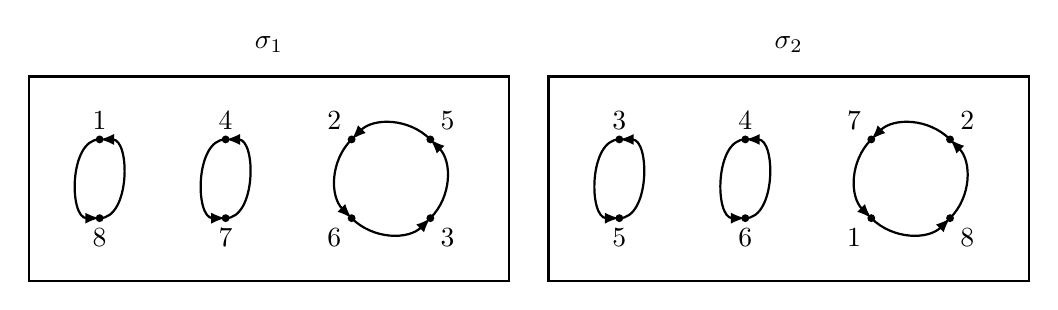
\begin{tikzpicture}[>=latex,thick]
\begin{scope}[xshift=-3.3cm]
\node at (-0.25,1.7) {$\sigma_1$};
\draw (-3.3,-1.3) rectangle (2.8,1.3);
\coordinate (A) at (-2.4,0.5);
\coordinate (B) at (-2.4,-0.5);
\coordinate (C) at (-0.8,0.5);
\coordinate (D) at (-0.8,-0.5);
\coordinate (E) at (0.8,0.5);
\coordinate (F) at (0.8,-0.5);
\coordinate (G) at (1.8,0.5);
\coordinate (H) at (1.8,-0.5);

\draw[->] (E) to[out=-135,in=135] (F);
\draw[->] (F) to[out=-45,in=-135] (H);
\draw[->] (H) to[out=45,in=-45] (G);
\draw[->] (G) to[out=135,in=45] (E);

\draw[->] (A) to[out=-180,in=-180] (B);
\draw[->] (B) to[out=0,in=0] (A);

\draw[->] (C) to[out=-180,in=-180] (D);
\draw[->] (D) to[out=0,in=0] (C);

\node at (A) [above] {$1$};
\node at (B) [below] {$8$};
\node at (C) [above] {$4$};
\node at (D) [below] {$7$};
\node at (E) [above left] {$2$};
\node at (F) [below left] {$6$};
\node at (H) [below right] {$3$};
\node at (G) [above right] {$5$};

\fill (A) circle[radius=0.05];
\fill (B) circle[radius=0.05];
\fill (C) circle[radius=0.05];
\fill (D) circle[radius=0.05];
\fill (E) circle[radius=0.05];
\fill (F) circle[radius=0.05];
\fill (G) circle[radius=0.05];
\fill (H) circle[radius=0.05];
\end{scope}
\begin{scope}[xshift=3.3cm]
\node at (-0.25,1.7) {$\sigma_2$};
\draw (-3.3,-1.3) rectangle (2.8,1.3);
\coordinate (A) at (-2.4,0.5);
\coordinate (B) at (-2.4,-0.5);
\coordinate (C) at (-0.8,0.5);
\coordinate (D) at (-0.8,-0.5);
\coordinate (E) at (0.8,0.5);
\coordinate (F) at (0.8,-0.5);
\coordinate (G) at (1.8,0.5);
\coordinate (H) at (1.8,-0.5);

\draw[->] (E) to[out=-135,in=135] (F);
\draw[->] (F) to[out=-45,in=-135] (H);
\draw[->] (H) to[out=45,in=-45] (G);
\draw[->] (G) to[out=135,in=45] (E);

\draw[->] (A) to[out=-180,in=-180] (B);
\draw[->] (B) to[out=0,in=0] (A);

\draw[->] (C) to[out=-180,in=-180] (D);
\draw[->] (D) to[out=0,in=0] (C);

\node at (A) [above] {$3$};
\node at (B) [below] {$5$};
\node at (C) [above] {$4$};
\node at (D) [below] {$6$};
\node at (E) [above left] {$7$};
\node at (F) [below left] {$1$};
\node at (H) [below right] {$8$};
\node at (G) [above right] {$2$};

\fill (A) circle[radius=0.05];
\fill (B) circle[radius=0.05];
\fill (C) circle[radius=0.05];
\fill (D) circle[radius=0.05];
\fill (E) circle[radius=0.05];
\fill (F) circle[radius=0.05];
\fill (G) circle[radius=0.05];
\fill (H) circle[radius=0.05];
\end{scope}
\end{tikzpicture}
\end{center}
Da die beiden Permutationen die gleiche Zyklenzerlegung haben, müssen
sie konjugiert sein.
Die Permutation
\[
\gamma
=
\begin{pmatrix}
1&2&3&4&5&6&7&8\\
6&5&1&4&8&7&2&3
\end{pmatrix}
\]
bildet die Zyklenzerlegung ab, also ist $\gamma\sigma_1\gamma^{-1}=\sigma_2$.
\end{loesung}
